\documentclass[border=4pt]{standalone}
\usepackage{amsmath,amssymb}
\usepackage{tikz,tikz-3dplot}
\usetikzlibrary{arrows.meta,calc}
\begin{document}
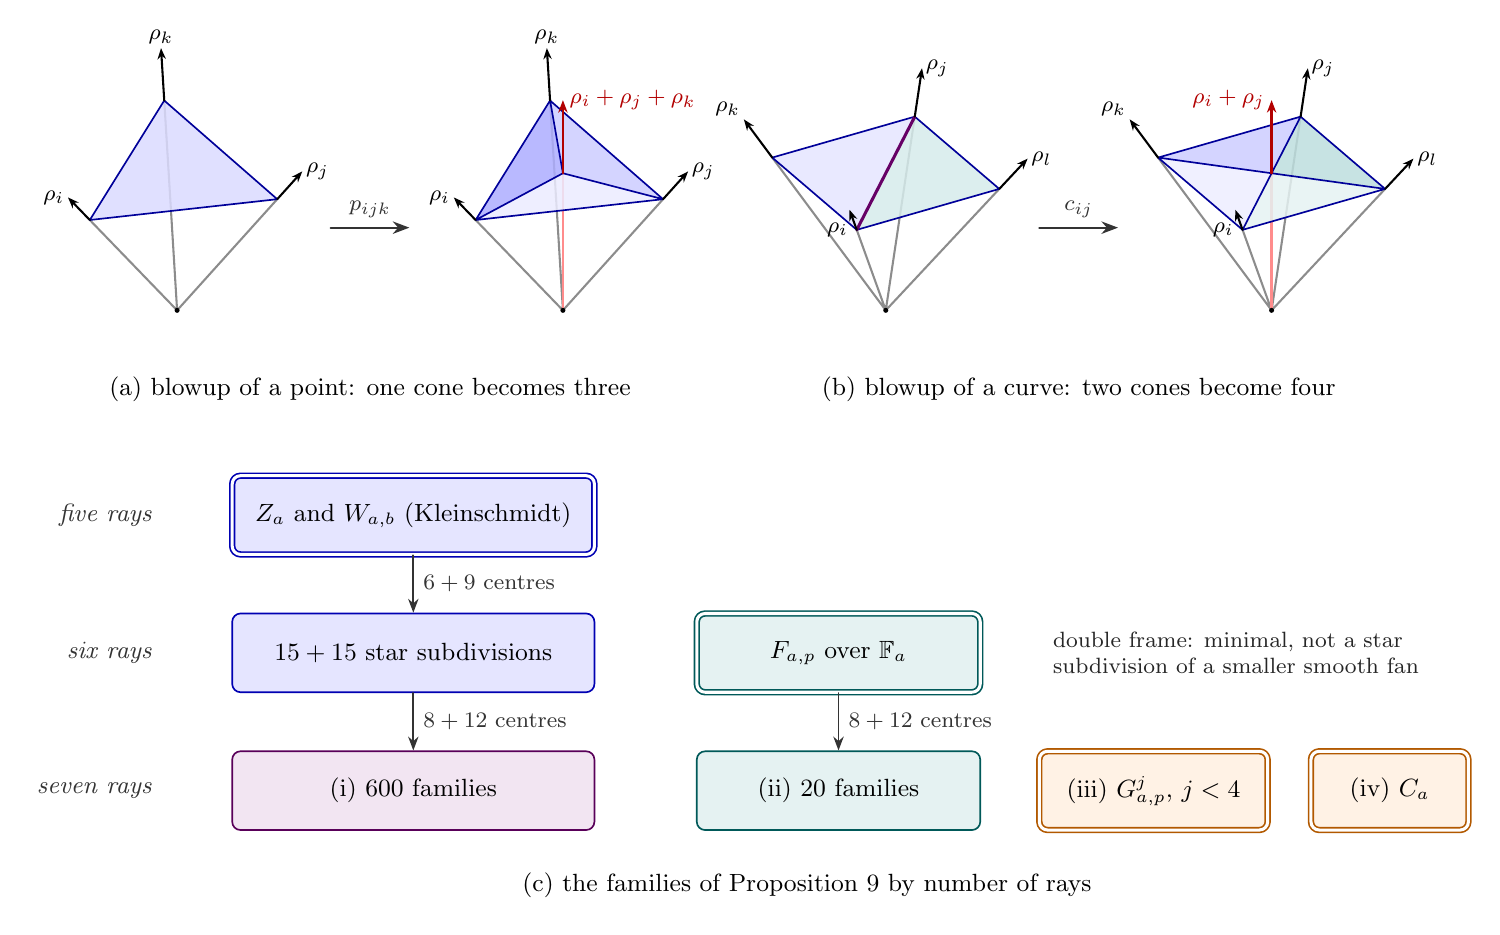
\begin{tikzpicture}[line join=round,line cap=round,
  ray/.style={line width=0.75pt,-{Stealth[length=4pt]}},
  inner/.style={line width=0.75pt,black!45},
  newray/.style={line width=0.9pt,red!70!black,-{Stealth[length=4.5pt]}},
  lab/.style={font=\footnotesize,inner sep=1pt},
  blowstep/.style={-{Stealth[length=6pt]},line width=0.8pt,gray!40!black}]
\tdplotsetmaincoords{56}{112}
% ---------- (a) a three-dimensional cone and p_{ijk} ----------
\begin{scope}[tdplot_main_coords,scale=0.7]
  \coordinate (O) at (0,0,0);
  \coordinate (A) at (2.0,-0.9,3); \coordinate (B) at (0.1,2.0,3); \coordinate (C) at (-2.1,-1.1,3);
  \draw[inner] (O)--(A) (O)--(B) (O)--(C);
  \fill[blue!14,fill opacity=0.85] (A)--(B)--(C)--cycle;
  \draw[blue!60!black,line width=0.6pt] (A)--(B)--(C)--cycle;
  \foreach \P/\n/\pos in {A/i/left,B/j/right,C/k/above}
    \draw[ray] (\P)--($(O)!1.25!(\P)$) node[lab,\pos]{$\rho_\n$};
  \fill (O) circle (1.3pt);
\end{scope}
\draw[blowstep] (1.95,1.05)--node[above,font=\footnotesize]{$p_{ijk}$} (2.95,1.05);
\begin{scope}[xshift=4.9cm,tdplot_main_coords,scale=0.7]
  \coordinate (O) at (0,0,0);
  \coordinate (A) at (2.0,-0.9,3); \coordinate (B) at (0.1,2.0,3); \coordinate (C) at (-2.1,-1.1,3);
  \coordinate (G) at (0,0,3);
  \draw[inner] (O)--(A) (O)--(B) (O)--(C);
  \draw[line width=0.9pt,red!45] (O)--(G);
  \begin{scope}[fill opacity=0.85]
  \fill[blue!8] (A)--(B)--(G)--cycle;
  \fill[blue!20] (B)--(C)--(G)--cycle;
  \fill[blue!32] (C)--(A)--(G)--cycle;
  \end{scope}
  \draw[blue!60!black,line width=0.6pt] (A)--(B)--(C)--cycle (A)--(G) (B)--(G) (C)--(G);
  \foreach \P/\n/\pos in {A/i/left,B/j/right,C/k/above}
    \draw[ray] (\P)--($(O)!1.25!(\P)$) node[lab,\pos]{$\rho_\n$};
  \draw[newray] (G)--(0,0,4.6) node[lab,right=1pt,red!70!black]{$\rho_i+\rho_j+\rho_k$};
  \fill (O) circle (1.3pt);
\end{scope}
\node[font=\small] at (2.45,-1.0) {(a) blowup of a point: one cone becomes three};
% ---------- (b) two cones along a common face and c_{ij} ----------
\begin{scope}[xshift=9.0cm,tdplot_main_coords,scale=0.7]
  \coordinate (O) at (0,0,0);
  \coordinate (I) at (1.9,0.2,3); \coordinate (J) at (-1.9,-0.2,3);
  \coordinate (K) at (0.3,-2.1,3); \coordinate (L) at (-0.3,2.1,3);
  \draw[inner] (O)--(I) (O)--(J) (O)--(K) (O)--(L);
  \begin{scope}[fill opacity=0.85]
  \fill[blue!10] (I)--(J)--(K)--cycle;
  \fill[teal!16] (I)--(J)--(L)--cycle;
  \end{scope}
  \draw[blue!60!black,line width=0.6pt] (I)--(K)--(J)--(L)--cycle;
  \draw[line width=1.1pt,violet!80!black] (I)--(J);
  \foreach \P/\n/\pos in {J/j/right,K/k/above left,L/l/right}
    \draw[ray] (\P)--($(O)!1.25!(\P)$) node[lab,\pos]{$\rho_\n$};
  \draw[ray] (I)--($(O)!1.25!(I)$);
  \node[lab,left=2pt] at (I) {$\rho_i$};
  \fill (O) circle (1.3pt);
\end{scope}
\draw[blowstep] (10.95,1.05)--node[above,font=\footnotesize]{$c_{ij}$} (11.95,1.05);
\begin{scope}[xshift=13.9cm,tdplot_main_coords,scale=0.7]
  \coordinate (O) at (0,0,0);
  \coordinate (I) at (1.9,0.2,3); \coordinate (J) at (-1.9,-0.2,3);
  \coordinate (K) at (0.3,-2.1,3); \coordinate (L) at (-0.3,2.1,3);
  \coordinate (M) at (0,0,3);
  \draw[inner] (O)--(I) (O)--(J) (O)--(K) (O)--(L);
  \draw[line width=0.9pt,red!45] (O)--(M);
  \begin{scope}[fill opacity=0.85]
  \fill[blue!7] (I)--(M)--(K)--cycle;   \fill[blue!20] (M)--(J)--(K)--cycle;
  \fill[teal!10] (I)--(M)--(L)--cycle;  \fill[teal!26] (M)--(J)--(L)--cycle;
  \end{scope}
  \draw[blue!60!black,line width=0.6pt] (I)--(K)--(J)--(L)--cycle (I)--(J) (K)--(M) (M)--(L);
  \foreach \P/\n/\pos in {J/j/right,K/k/above left,L/l/right}
    \draw[ray] (\P)--($(O)!1.25!(\P)$) node[lab,\pos]{$\rho_\n$};
  \draw[ray] (I)--($(O)!1.25!(I)$);
  \node[lab,left=2pt] at (I) {$\rho_i$};
  \draw[newray] (M)--(0,0,4.6) node[lab,left=1pt,red!70!black]{$\rho_i+\rho_j$};
  \fill (O) circle (1.3pt);
\end{scope}
\node[font=\small] at (11.45,-1.0) {(b) blowup of a curve: two cones become four};
% ---------- (c) where the 625 families come from ----------
\begin{scope}[yshift=-2.6cm,
  fam/.style={draw=#1!70!black,fill=#1!10,rounded corners=3pt,line width=0.6pt,
              align=center,font=\small,inner sep=4pt,minimum height=10mm},
  fam/.default=gray,
  minimal/.style={double,double distance=1.1pt},
  arr/.style={-{Stealth[length=5pt]},line width=0.6pt,gray!40!black},
  row/.style={font=\small\itshape,anchor=east,text=gray!40!black}]
  \node[row] at (-0.2,0) {five rays};
  \node[row] at (-0.2,-1.75) {six rays};
  \node[row] at (-0.2,-3.5) {seven rays};
  \node[fam=blue,minimal,minimum width=4.6cm] (Z) at (3.0,0)
     {$Z_a$ and $W_{a,b}$ (Kleinschmidt)};
  \node[fam=blue,minimum width=4.6cm] (Z1) at (3.0,-1.75)
     {$15+15$ star subdivisions};
  \node[fam=teal,minimal,minimum width=3.6cm] (F) at (8.4,-1.75)
     {$F_{a,p}$ over $\mathbb{F}_a$};
  \node[fam=violet,minimum width=4.6cm] (i) at (3.0,-3.5)
     {(i) $600$ families};
  \node[fam=teal,minimum width=3.6cm] (ii) at (8.4,-3.5)
     {(ii) $20$ families};
  \node[fam=orange,minimal,minimum width=2.9cm] (iii) at (12.4,-3.5)
     {(iii) $G^j_{a,p}$, $j<4$};
  \node[fam=orange,minimal,minimum width=2.0cm] (iv) at (15.4,-3.5)
     {(iv) $C_a$};
  \draw[arr] (Z) -- node[right,font=\footnotesize]{$6+9$ centres} (Z1);
  \draw[arr] (Z1) -- node[right,font=\footnotesize]{$8+12$ centres} (i);
  \draw[arr] (F) -- node[right,font=\footnotesize]{$8+12$ centres} (ii);
  \node[font=\footnotesize,align=left,text=gray!30!black,anchor=west] at (11.0,-1.75)
     {double frame: minimal, not a star\\subdivision of a smaller smooth fan};
\end{scope}
\node[font=\small] at (8.0,-7.3) {(c) the families of Proposition 9 by number of rays};
\end{tikzpicture}
\end{document}
